\section{Deep Embedded Clustering with Consensus Representations (DECCS)}

The DECCS paper \citep{Miklautz2021}, "Deep Clustering With Consensus Representations," presents an innovative approach in the field of deep clustering. It addresses the limitations of existing deep clustering methods that are typically designed for a single clustering model, like k-means, spectral clustering, or Gaussian mixture models. These methods often fall short when their underlying assumptions are not met by the data.

DECCS (Deep Embedded Clustering with Consensus Representations) proposes a novel method that combines deep learning and clustering to improve both the learned representation and the performance of multiple heterogeneous clustering algorithms simultaneously. This approach is a significant departure from current deep clustering (DC) and consensus clustering (CC) methods, which typically focus on single models and may not effectively handle high-dimensional datasets or non-linear transformations.

\subsection{Related Work in Consensus Clustering and Deep Clustering}

\begin{itemize}
\item \textbf{Consensus Clustering (CC):} Traditional CC methods create robust clustering by combining multiple solutions into a single partition. However, they often don't access the original data features and are limited to linear transformations or specific clustering types like k-means. DECCS overcomes these limitations by learning a non-linear consensus function for the representation as follows:

\begin{itemize}
    \item \(\Theta\) - Set of learnable parameters of the encoder.
    \item \textit{enc} - Encoder function that maps data points to a lower-dimensional embedded space.
    \item \(X\) - An \(N \times D\) dimensional input data matrix.
    \item \(Z\) - An \(N \times d\) dimensional embedded data matrix, where \(Z = \textit{enc}(X)\) and \(d < D\).
    \item \(\mathcal{E}\) - Set of heterogeneous clustering algorithms.
    \item \(k_i\) - Number of clusters for the \(i^{th}\) clustering algorithm \(e_i\).
    \item \(\pi_i\) - Clustering result for the \(i^{th}\) clustering algorithm, where \(\pi_i = e_i(Z)\).
    \item \(Z_{cr}\) - Consensus representation that maximizes the objective function involving normalized mutual information across clustering results.
    \item \(c\) - Normalization constant for the objective function, defined as \(c = \frac{2}{|\mathcal{E}|^2-|\mathcal{E}|}\) to ensure the equation sums to one.
    \item \(f_{\Theta}\) - Objective function for consensus representation.
    \item \(NMI\) - Normalized Mutual Information, used as a measure in the objective function.
\end{itemize}

\(Z_{cr}\) maximizes the following objective function:

\[
f_{\Theta} = c \sum_{i=1}^{|\mathcal{E}|} \sum_{j>i}^{|\mathcal{E}|} NMI(e_i(\textit{enc}(\Theta)(X)), e_j(\textit{enc}(\Theta)(X))),
\]
where
\[
Z_{cr} := \textit{enc}_{\Theta_{cr}}(X),
\]
and \(\textit{enc}_{\Theta_{cr}}\) is the \textit{consensus representation function} and \(c\) is a normalization constant
\[
c = \frac{2}{|\mathcal{E}|^2-|\mathcal{E}|}
\]
for the equation to sum to one.

\item \textbf{Deep Clustering (DC):} Existing DC methods are typically tailored to a single clustering model, which may not always align with the data's characteristics. Methods like SpectralNet, DEC, and VaDE focus on specific clustering algorithms but do not account for the diversity of data types and clustering requirements found in complex datasets. For instance, DEC \citep{Xie2016} introduces a novel approach to clustering by combining representation learning with clustering in a deep learning framework. DEC uses a deep neural network to learn a mapping from the data space to a lower-dimensional feature space, where clustering is performed. The DEC algorithm iteratively refines cluster centers using a clustering loss function, significantly improving clustering results on various datasets. However, DEC struggles with handling different types of data and may not provide satisfactory results for highly heterogeneous datasets.

\item \textbf{Variational Autoencoders (VAE):} Introduced by Kingma and Welling (2014) \citep{Kingma2014}, VAE is a powerful generative model that learns a probabilistic mapping from data to a latent space and back. VAEs combine principles from variational inference and deep learning, making them effective for learning complex data distributions and generating new data samples. The VAE framework consists of an encoder that maps input data to a latent space and a decoder that reconstructs the data from the latent space. VAEs are particularly useful in clustering because they create smooth and continuous latent spaces where similar data points remain close in the latent space, thus facilitating improved clustering performance. However, VAEs also face limitations in dealing with the variability and complexity of real-world data.
\end{itemize}

\subsection{Methodology of DECCS}

DECCS is innovative in using a consensus representation learning approach, where it employs an autoencoder (AE) to learn a simplified representation of data. This simplification reduces ambiguity and increases the similarity of clustering results across different ensemble members, thus improving the overall clustering performance. The method involves three main steps: generating base partitions, approximating each partition with a classifier, and then updating the consensus representation.

\begin{figure}
\centering
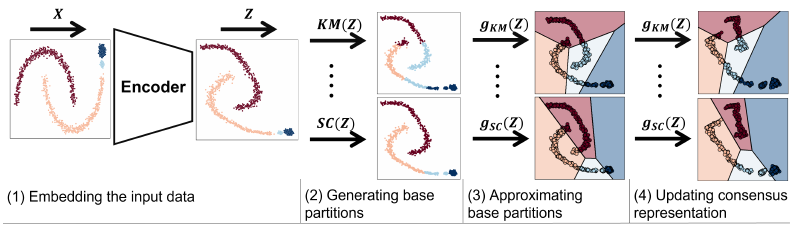
\includegraphics[width=1\textwidth]{figs/deccs.png}
    \caption{Visualisation of one round of DECCS\citep{Miklautz2021}. (1) The encoder is used to embed data points $X$. (2) Clustering results are generated by applying ensemble members $\mathcal{E} = \{KM, \ldots, SC\}$ to $Z$. (3) Classifiers $g_i$ are trained to predict the corresponding cluster labels $\pi_i$ from $Z$. (4) $Z$ is updated via minimizing $\mathcal{L}$.}
\label{fig:pipeline}
\end{figure}

\subsection{Experimental Evaluation}

DECCS was evaluated across various datasets, including MNIST, Fashion-MNIST, Kuzushiji-MNIST, USPS, and others. The experimental setup involved using a feed-forward AE architecture and setting specific hyperparameters for DECCS, like the consensus weight (cons) and sampling size (n). The evaluation metrics included normalized mutual information (NMI) and adjusted rand index (ARI), focusing on the agreement within an ensemble and cluster performance. DECCS showed improved agreement and cluster performance across all ensemble members, outperforming several relevant baselines from deep clustering and consensus clustering.

In summary, DECCS represents a significant advancement in deep clustering, effectively addressing the challenges of integrating multiple clustering methods. Its ability to learn a consensus representation that maximizes ensemble agreement marks a key innovation in this field.

\section{Deep Descriptive Clustering (DDC)}

The paper "Deep Descriptive Clustering" \citep{Zhang2021} by Hongjing Zhang and Ian Davidson explores a novel approach to clustering complex data such as images, text, and graphs, with a focus on explainable AI (XAI). This approach is particularly significant in the context of unsupervised learning like clustering, where explanations are crucial at the model level rather than just the instance level. The paper introduces the Deep Descriptive Clustering (DDC) framework, which combines deep clustering with cluster-level explanations. This framework is unique in its ability to learn from both sub-symbolic (clustering) and symbolic (explanation) levels simultaneously.

\subsection{Key Aspects of Deep Descriptive Clustering (DDC)}

\textbf{Clustering Objective:} DDC maximizes the mutual information between the empirical distribution on the inputs and the induced clustering labels. This approach is inspired by the discriminative clustering model, which has fewer assumptions about the data.

\textbf{Class-Level Explanation Objective:} DDC uses Integer Linear Programming (ILP) to generate concise and orthogonal explanations for each cluster. This method addresses the limitations of existing approaches that either require interpretable features or are post-hoc explanations that don't inform the clustering process.

\textbf{Self-Generated Pairwise Loss Term:} This innovative component reconciles inconsistencies between clustering and explanation by introducing self-generated constraints. The method leverages semantic tags to generate explanations and reshape clustering features, improving the overall clustering quality.

\begin{figure}
\centering
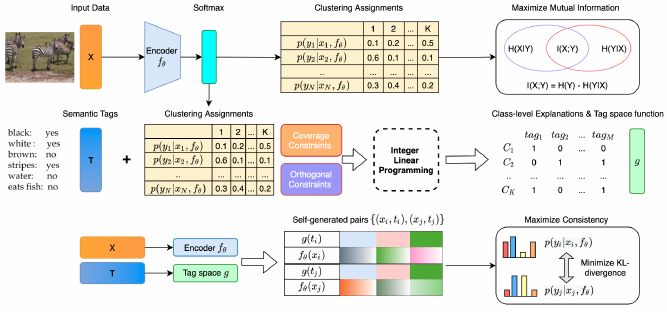
\includegraphics[width=1\textwidth]{figs/dec.png}
    \caption{The framework of deep descriptive clustering (DDC). DDC consists of one clustering objective, one sub-symbolic explanation objective, and one self-generated objective to maximize the consistency between clustering and explanation modules.}
\label{fig:ddc}
\end{figure}

\subsection{Experiments and Findings}

The paper evaluates the DDC framework on datasets like Attribute Pascal and Yahoo (aPY) and Animals with Attributes (AwA), comparing it against other methods in terms of explanation quality and clustering performance. DDC outperforms competitive baselines in clustering performance and offers high-quality cluster-level explanations. The evaluation metrics used include Tag Coverage (TC) and Inverse Tag Frequency (ITF), along with Normalized Mutual Information (NMI) and Clustering Accuracy (ACC) for a comprehensive assessment.

\subsection{Conclusion and Future Directions}

The paper concludes that the deep descriptive clustering model successfully clusters and generates high-quality cluster-level explanations. It emphasizes the model's potential in dealing with noisy semantic features and exploring novel forms of explanations beyond ontologies. Future work is directed towards enhancing the explainability of clustering models in diverse data contexts. In summary, this paper presents a groundbreaking approach in the field of explainable AI, offering a robust framework for both clustering and generating meaningful explanations.

\section{Related Works}

\subsection{Deep Embedded Clustering: A General Approach to Clustering Arbitrary Similarity Measures by J. Xie, R. Girshick, and A. Farhadi (2016)}

Deep Embedded Clustering (DEC) is a seminal work by Xie, Girshick, and Farhadi (2016) that introduces a novel approach to clustering by combining representation learning with clustering in a deep learning framework. DEC uses a deep neural network to learn a mapping from the data space to a lower-dimensional feature space, where clustering is performed. The key innovation of DEC is its use of an unsupervised learning algorithm that iteratively refines the cluster centers and improves clustering quality through a clustering loss function.

The DEC algorithm involves two main steps: the initial embedding of data into a lower-dimensional space using a stacked autoencoder, and the subsequent clustering of these embeddings using a clustering objective that minimizes the Kullback-Leibler (KL) divergence between the soft assignments and a target distribution. This iterative process allows the algorithm to refine both the embeddings and the cluster centers, resulting in better clustering performance.

DEC has been shown to significantly improve clustering results on various datasets compared to traditional methods, establishing its effectiveness and robustness. This work is foundational in demonstrating the power of deep learning for clustering tasks, and it has inspired numerous subsequent studies in the field of deep clustering \citep{Xie2016}.

\begin{figure}[h]
    \centering
    %\includegraphics[width=0.8\textwidth]{dec_architecture.png}
    \caption{Architecture of the Deep Embedded Clustering (DEC) model. The model consists of a stacked autoencoder followed by a clustering layer. The autoencoder learns a low-dimensional representation of the data, which is then clustered using a clustering objective.}
    \label{fig:dec_architecture}
\end{figure}

\subsection{Auto-Encoding Variational Bayes by D. P. Kingma and M. Welling (2014)}

Auto-Encoding Variational Bayes (VAE) is a powerful generative model introduced by Kingma and Welling (2014) that learns a probabilistic mapping from data to a latent space and back. VAEs combine principles from variational inference and deep learning, making them highly effective for learning complex data distributions and generating new data samples.

The VAE framework consists of two main components: an encoder that maps the input data to a latent space, and a decoder that reconstructs the data from the latent space. The encoder produces parameters for a probability distribution in the latent space, typically Gaussian, from which latent variables are sampled. The decoder then reconstructs the input data from these latent variables. The training objective of a VAE includes a reconstruction loss, which ensures the reconstructed data is similar to the original data, and a regularization term, which ensures the latent space distribution is close to a prior distribution, typically Gaussian.

VAEs are particularly useful in clustering because they create smooth and continuous latent spaces where data points that are similar in the original space remain close in the latent space. This property makes it easier to apply clustering algorithms to the latent representations learned by the VAE, leading to improved clustering performance \citep{Kingma2014}.

\begin{figure}[h]
    \centering
%    \includegraphics[width=0.8\textwidth]{vae_architecture.png}
    \caption{Architecture of the Variational Autoencoder (VAE) model. The encoder maps input data to a latent space, and the decoder reconstructs the data from the latent space. The model is trained to minimize reconstruction loss and regularization loss.}
    \label{fig:vae_architecture}
\end{figure}

\subsection{Explainable-by-Design Algorithms}

Explainable-by-design algorithms, as conceptualized by researchers like Bertsimas et al. (2020) and Moshkovitz et al. (2020), represent a class of methods that inherently integrate interpretability into the clustering process. These algorithms are designed with a dual purpose: to perform clustering tasks and simultaneously provide understandable explanations for the clustering outcomes. By utilizing interpretable features, such as simple and easily understandable attributes, these methods ensure that both the process and results of clustering are transparent and comprehensible to users.

The fundamental approach of these algorithms is to employ interpretable features in the construction of decision trees or other similar models, which then serve as the basis for both clustering and explaining the grouped data. For instance, in a clustering task involving customer segmentation, an explainable-by-design algorithm might use customer attributes like age, location, or purchasing habits, which are inherently interpretable, to form clusters and provide explanations for why certain customers are grouped together.

However, the application of these algorithms has certain limitations, particularly when dealing with complex data types such as images or graphs. In such scenarios, the raw features (like pixel values in images or edge connections in graphs) are often high-dimensional, less interpretable, and do not lend themselves to straightforward explanations. This limitation restricts the effectiveness of explainable-by-design algorithms in scenarios where the data complexity exceeds the interpretability of the features used for clustering.

\subsection{Post-processing Explanation Methods}

Post-processing explanation methods, developed by researchers like Davidson et al. (2018) and Sambaturu et al. (2020) \citep{Sambaturu2020}, take a different approach to explainability in clustering. Unlike explainable-by-design algorithms, these methods do not integrate explainability into the clustering process itself. Instead, they focus on generating explanations for pre-existing clustering results. These methods typically employ an additional set of features, often referred to as semantic tags, which are used to post-process and explain the outcomes of the clustering algorithms.

For example, in a clustering task involving document classification, a post-processing method might use semantic tags related to the content or theme of the documents to provide explanations for why certain documents are grouped together. This approach is algorithm-agnostic, meaning it can be applied to the results of any clustering algorithm, regardless of how the initial clustering was performed.

However, a critical limitation of post-processing explanation methods is that they may not fully leverage the information available from the additional features. Since these methods are applied after the clustering has been completed, they often rely on the inherent quality of the initial clustering. If the original clustering does not align well with the semantic tags used for explanation, the resulting explanations can be suboptimal or less meaningful. This disconnect between the clustering process and the post-hoc explanation phase can lead to explanations that do not fully capture the nuances or the rationale behind the formed clusters.

\subsection{Other Related Works}

Other significant contributions to the field of interpretable clustering include the works by Rishinanda and Sebag (2021) on deep discriminative clustering analysis, Liu et al. (2022) on generating natural language descriptions for clusters, and Chhajer and Moniri (2022) on using disentangled representations for clustering. These studies have advanced the understanding of how deep learning techniques can be leveraged to improve both the performance and interpretability of clustering algorithms.

Rishinanda and Sebag (2021) propose a deep learning approach that combines representation learning and discriminative clustering, aiming to produce well-separated and interpretable clusters. Liu et al. (2022) introduce a framework for generating natural language descriptions for clusters, enhancing the accessibility of clustering results to non-experts. Chhajer and Moniri (2022) focus on disentangled representations, which separate different explanatory factors in the data, making the clustering results more understandable.

These advancements demonstrate the ongoing efforts to make clustering algorithms not only more accurate but also more interpretable, bridging the gap between complex data analysis and human understanding \cite{Rishinanda2021, Liu2022, Chhajer2022}.